\section{Training Paradigm}

\begin{figure}[t]
    \centering
    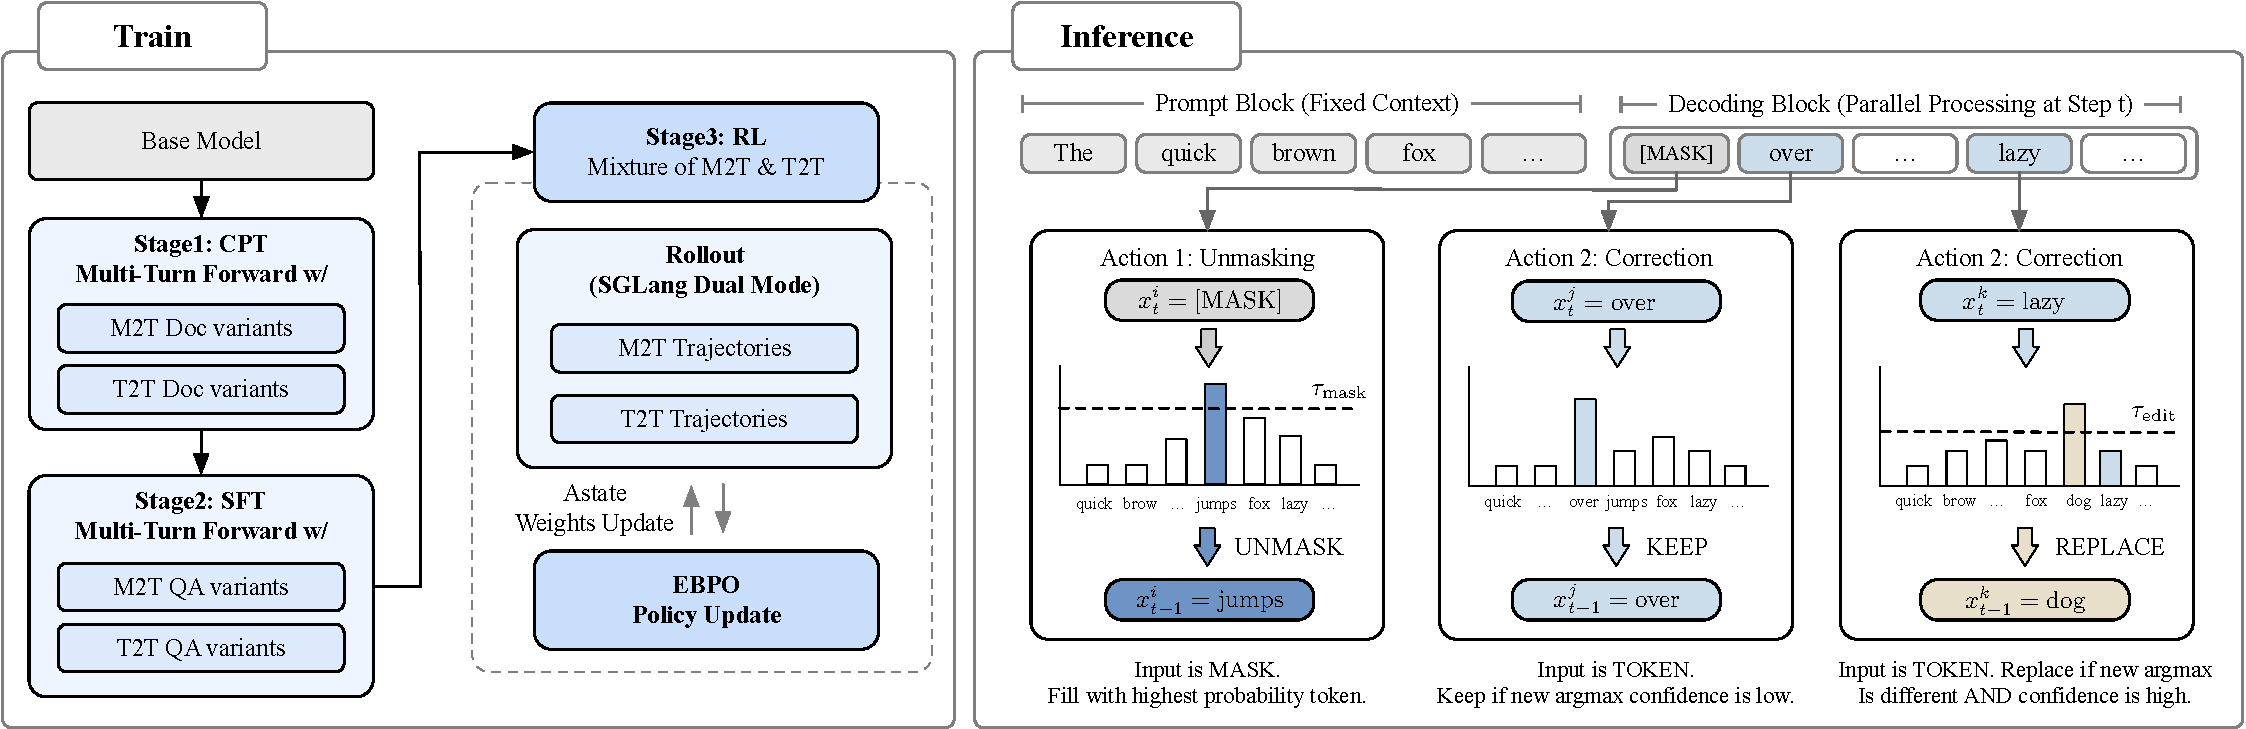
\includegraphics[width=\linewidth]{images/framework}
    \caption{Overview of training \& inference framework of LLaDA2.1}
    \label{fig:framework}
\end{figure}

\subsection{Training Alignment for ``Draft-and-Edit"}
To align the model with the ``Draft-and-Edit" inference paradigm and mitigate the \emph{Exposure Bias} inherent in standard mask-based training, we employ a unified \textbf{Mixture of M2T and T2T} objective. This objective is applied throughout both the Continual Pre-Training (CPT) and Supervised Finetuning (SFT) stages.

This dual-stream training objective enables the model to develop two complementary capabilities fundamental to our framework:

\begin{itemize} 
\item \textbf{Drafting Stream (Mask-to-Token):} 
The model learns to predict the correct token at each masked position to generate initial content, establishing the foundational drafting capability. 

\item \textbf{Editing Stream (Token-to-Token):} 
The model learns to recover original tokens from random noise perturbations (rectifying errors), equipping it with the ability to identify and rewrite artifacts. 
\end{itemize}


By consistently applying this dual-stream supervision from CPT through SFT, we ensure that LLaDA2.1 is fundamentally conditioned to function as both a fast drafter and a precise editor within a single parameter space. Additionally, we employ a Multi-turn Forward (MTF) data augmentation technique, by exposing the model to a wider variety of editing scenarios, enhance the model's editing capabilities.